\documentclass{article}\usepackage[]{graphicx}\usepackage[]{color}
%% maxwidth is the original width if it is less than linewidth
%% otherwise use linewidth (to make sure the graphics do not exceed the margin)
\makeatletter
\def\maxwidth{ %
  \ifdim\Gin@nat@width>\linewidth
    \linewidth
  \else
    \Gin@nat@width
  \fi
}
\makeatother

\definecolor{fgcolor}{rgb}{0.345, 0.345, 0.345}
\newcommand{\hlnum}[1]{\textcolor[rgb]{0.686,0.059,0.569}{#1}}%
\newcommand{\hlstr}[1]{\textcolor[rgb]{0.192,0.494,0.8}{#1}}%
\newcommand{\hlcom}[1]{\textcolor[rgb]{0.678,0.584,0.686}{\textit{#1}}}%
\newcommand{\hlopt}[1]{\textcolor[rgb]{0,0,0}{#1}}%
\newcommand{\hlstd}[1]{\textcolor[rgb]{0.345,0.345,0.345}{#1}}%
\newcommand{\hlkwa}[1]{\textcolor[rgb]{0.161,0.373,0.58}{\textbf{#1}}}%
\newcommand{\hlkwb}[1]{\textcolor[rgb]{0.69,0.353,0.396}{#1}}%
\newcommand{\hlkwc}[1]{\textcolor[rgb]{0.333,0.667,0.333}{#1}}%
\newcommand{\hlkwd}[1]{\textcolor[rgb]{0.737,0.353,0.396}{\textbf{#1}}}%
\let\hlipl\hlkwb

\usepackage{framed}
\makeatletter
\newenvironment{kframe}{%
 \def\at@end@of@kframe{}%
 \ifinner\ifhmode%
  \def\at@end@of@kframe{\end{minipage}}%
  \begin{minipage}{\columnwidth}%
 \fi\fi%
 \def\FrameCommand##1{\hskip\@totalleftmargin \hskip-\fboxsep
 \colorbox{shadecolor}{##1}\hskip-\fboxsep
     % There is no \\@totalrightmargin, so:
     \hskip-\linewidth \hskip-\@totalleftmargin \hskip\columnwidth}%
 \MakeFramed {\advance\hsize-\width
   \@totalleftmargin\z@ \linewidth\hsize
   \@setminipage}}%
 {\par\unskip\endMakeFramed%
 \at@end@of@kframe}
\makeatother

\definecolor{shadecolor}{rgb}{.97, .97, .97}
\definecolor{messagecolor}{rgb}{0, 0, 0}
\definecolor{warningcolor}{rgb}{1, 0, 1}
\definecolor{errorcolor}{rgb}{1, 0, 0}
\newenvironment{knitrout}{}{} % an empty environment to be redefined in TeX

\usepackage{alltt}
\documentclass{article}
\documentclass{article}

\usepackage{amsmath, amsthm, amssymb}
\usepackage[round]{natbib}

% The line below tells R to use knitr on this.
%\VignetteEngine{knitr::knitr}

\title{An R package for Newton's Algorithm}
\author{Robin Hood \and Maid Marion \and Will Scarlett}
\IfFileExists{upquote.sty}{\usepackage{upquote}}{}
\begin{document}
\SweaveOpts{concordance=TRUE}

\maketitle

\begin{abstract}
We present the R package `testpkg', which does some useful things.
\end{abstract}

\section{Introduction}

Here is a nice description of the background.

Suppose we wish to find the root of the function $f(x) = x^3 - x - 1$, which lies
between 1 and 2.
% below is a code chunk. You don't have to give it a name, but if you do
% it MUST be unique.
\begin{knitrout}
\definecolor{shadecolor}{rgb}{0.969, 0.969, 0.969}\color{fgcolor}\begin{kframe}
\begin{alltt}
\hlstd{f} \hlkwb{=} \hlkwa{function}\hlstd{(}\hlkwc{x}\hlstd{) x}\hlopt{^}\hlnum{3} \hlopt{-} \hlstd{x} \hlopt{-} \hlnum{1}
\end{alltt}
\end{kframe}
\end{knitrout}
You can do plots and they'll automatically be added to your document.
\begin{knitrout}
\definecolor{shadecolor}{rgb}{0.969, 0.969, 0.969}\color{fgcolor}\begin{kframe}
\begin{alltt}
\hlkwd{plot}\hlstd{(f,} \hlnum{1}\hlstd{,} \hlnum{2}\hlstd{)}
\end{alltt}
\end{kframe}
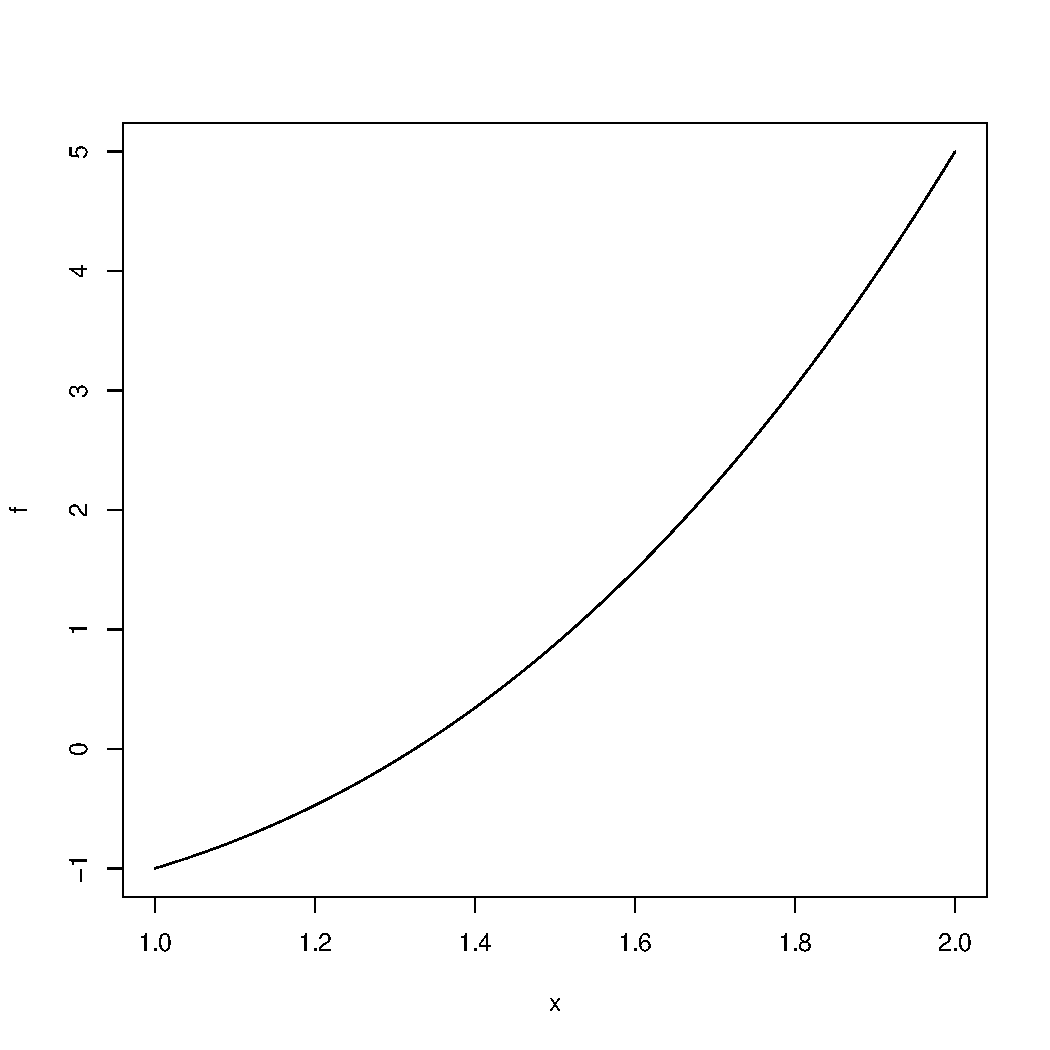
\includegraphics[width=\maxwidth]{figure/chunkname2-1} 

\end{knitrout}

\section{A Bit About knitr}

The code chunks you put in don't have to be displayed (and nor does the output),
if they are displayed they don't have to be evalutated.  To the next chunk I added
the option \verb|eval=FALSE|
\begin{knitrout}
\definecolor{shadecolor}{rgb}{0.969, 0.969, 0.969}\color{fgcolor}\begin{kframe}
\begin{alltt}
\hlkwd{rnorm}\hlstd{(}\hlnum{1e6}\hlstd{)}
\end{alltt}
\end{kframe}
\end{knitrout}
This code is evaluated, I just choose not to display the output:
\begin{knitrout}
\definecolor{shadecolor}{rgb}{0.969, 0.969, 0.969}\color{fgcolor}\begin{kframe}
\begin{alltt}
\hlnum{5}\hlopt{+}\hlnum{5}
\end{alltt}
\end{kframe}
\end{knitrout}
And finally you might want your code to be evaluated but not displayed (useful for
changing options without displaying in your document):


\section{\LaTeX}

\LaTeX itself is complicated if you've never used it before, but I'm sure you'll
pick it up quickly: there are a lot of guides on the web.  I recommend using the
\texttt{align} environment (in the \texttt{amsmath} package) for displayed equations:
\begin{align*}
% lose the *'s if you want equation numbers
f(x) &= x^3 - x - 1\\
g(y) &= y^4 + 2y
\end{align*}

You can cite in two ways using the \texttt{natbib} package:
\citep{articlekey}
and
\citet{articlekey}.

% now generate the bibliography from file mybib.bib
\bibliographystyle{plainnat}
\bibliography{mybib}


\end{document}
